% ACM-style DSAA 2026 industry-track draft.
% Compile with: pdflatex -interaction=nonstopmode -halt-on-error DSAA2026_DARS_Industry_Submission.tex
\documentclass[sigconf,nonacm]{acmart}

\setcopyright{none}
\settopmatter{printacmref=false,printccs=false,printfolios=true}
\renewcommand\footnotetextcopyrightpermission[1]{}
\pagestyle{plain}

\usepackage{booktabs}
\usepackage{array}
\usepackage{tabularx}
\usepackage{graphicx}
\usepackage{subcaption}
\usepackage{amsmath}
\usepackage{enumitem}
\usepackage{xcolor}

\definecolor{darsPurple}{HTML}{6D28D9}
\definecolor{darsBlue}{HTML}{2563EB}
\definecolor{darsGreen}{HTML}{16A34A}
\definecolor{darsGray}{HTML}{475569}

\title[DARS for GATEWay]{DARS for GATEWay: Industry-Ready Adaptive Assessment with Dynamic Rating, Graph-Guided Remediation, and Calibrated Student Analytics}

\author{Sunil Kumar}
\affiliation{%
  \institution{GATEWay Adaptive Preparation Platform}
  \city{India}
  \country{India}
}
\email{}

\begin{abstract}
Adaptive learning products need ability estimates that are fast, stable, explainable, and useful for intervention. Classical Elo is operationally simple but depends on a fixed sensitivity parameter; Glicko-2 handles rating uncertainty but does not directly model educational context; deep knowledge tracing models improve prediction but are harder to deploy and explain in teacher-facing systems. This paper presents DARS, a Dynamic Adaptive Rating System integrated into GATEWay, a full-stack GATE DA preparation platform. DARS combines dynamic update factors, response-quality scoring, streak and momentum signals, graph-guided item routing, rapid-guess handling, and remediation-aware analytics. We report an industry-oriented implementation and a reproducible benchmark over a 220-student bot cohort containing 55,000 temporal interactions, 1,683 adaptive tests, 77,850 test-question rows, and 2,140 graph edges. A calibrated DARS$^+$ model evaluated on held-out students outperforms Glicko-2, fixed Elo, static rating, and raw DARS across Brier score, log loss, ROC AUC, accuracy, and calibration error. DARS$^+$ achieves Brier 0.2244, log loss 0.6393, ROC AUC 0.6319, and ECE 0.0062. The result is a deployable industry prototype and a research-ready evaluation framework for graph-aware adaptive assessment.
\end{abstract}

\keywords{adaptive learning, educational data mining, dynamic rating, Elo, Glicko-2, knowledge tracing, graph recommendation, remediation, learning analytics}

\begin{document}
\maketitle

\section{Industry Problem and Motivation}
GATE DA preparation platforms must do more than score tests. A production system must estimate student readiness, select the next useful question, explain why a question was served, detect low-quality responses, and help teachers identify learners needing intervention. These requirements create a tension between predictive performance and operational explainability. Neural knowledge tracing models are powerful, but classroom products often need transparent, low-latency, auditable updates after every response. Rating systems are simple and scalable, but standard Elo is sensitive to the choice of a fixed $K$.

Recent educational rating research reinforces this trade-off. Vermeiren et al. argue that fixed $K$ values either track ability changes quickly but become volatile, or remain stable but adapt too slowly; they propose dynamic $K$ adjustment to balance stability and flexibility in adaptive learning environments~\cite{vermeiren2025dynamic}. Deep Knowledge Tracing (DKT) showed that recurrent neural networks can model student learning without hand-coded domain knowledge and improve prediction across KT datasets~\cite{piech2015dkt}. GIKT further argues that question-skill graphs are important because question characteristics and high-order question-skill correlations are lost in purely skill-based models~\cite{yang2020gikt}. DARS is positioned between these families: it keeps the operational transparency of rating systems while adding graph, timing, remediation, and momentum signals motivated by educational data mining.

\section{GATEWay System Overview}
GATEWay is a full-stack adaptive GATE DA preparation platform implemented with React, TypeScript, Supabase, reusable analytics components, and reproducible notebook pipelines. The platform supports student authentication, course joining, practice tests, adaptive tests, assignment attempts, review screens, teacher dashboards, rosters, course management, and analytics.

The DARS layer is integrated as a backend intelligence component. It updates student ratings, classifies momentum, detects rapid guesses, routes graph-neighborhood questions, records remediation flags, and exports CSV datasets for research. The repository contains production-facing source modules and reproducible artifacts:

\begin{itemize}[leftmargin=*]
  \item \texttt{src/lib/darsRating.ts}: DARS rating update implementation;
  \item \texttt{src/lib/nextBestQuestionEngine.ts}: graph-guided recommendation;
  \item \texttt{scripts/generate-dars-datasets.mjs}: 220-student dataset generator;
  \item \texttt{DARS\_All\_Metrics\_Comparison.ipynb}: benchmark notebook;
  \item \texttt{datasets/dars/*.csv}: connected student, response, graph, and metric datasets.
\end{itemize}

\section{DARS Model}
\subsection{Expected Success}
For learner rating $R$ and item rating $R_q$, DARS uses an Elo-style expected success probability:
\begin{equation}
E(q)=\frac{1}{1+10^{(R_q^\ast-R)/400}},
\end{equation}
where $R_q^\ast$ can include graph-centrality calibration. This keeps the score interpretable: if a learner rating exceeds item rating, expected success rises.

\subsection{Performance Quality}
DARS replaces binary correctness with a continuous performance quality score. For a correct response:
\begin{equation}
P(q)=w_\tau\tau(q)+w_h(1-H(q))+w_\psi\psi(k),
\end{equation}
where $\tau(q)$ is time efficiency, $H(q)$ is hint or support usage, and $\psi(k)$ is streak quality. For an incorrect response:
\begin{equation}
P(q)=\min(\epsilon_f, 0.05\tau(q)).
\end{equation}
Thus two correct responses need not be equally informative: a confident, timely response during a stable streak is stronger evidence than a slow or anomalous response.

\subsection{Dynamic Update}
The learner update is:
\begin{equation}
\Delta R = K(n,\sigma^2)\phi(k)(P(q)-E(q))-\rho(q),
\end{equation}
where $K(n,\sigma^2)$ decays with practice count and recent uncertainty, $\phi(k)$ is a bounded streak multiplier, and $\rho(q)$ is a rapid-guess penalty. This structure directly follows the dynamic-$K$ motivation in recent Elo-based adaptive learning work while adding education-specific response quality.

\subsection{Graph-Guided Routing}
The question bank is represented as a directed graph $G=(V,E)$. Nodes are questions with subject, topic, difficulty, Elo, marks, and response-time attributes. Edges encode same-topic progression, prerequisites, and cross-domain bridges. Standard routing selects candidates from a bounded neighborhood:
\begin{equation}
N(q,k)=\{q'\in V:d_G(q,q')\leq k,\ q'\notin Q_{ans}\}.
\end{equation}
Remediation routing selects related but easier questions:
\begin{equation}
N_r(q_m,h)=\{q'\in V:d_G(q_m,q')\leq h,\ diff(q')<diff(q_m)\}.
\end{equation}
This design is consistent with graph-based KT literature: GIKT uses question-skill graph propagation to reduce sparsity and exploit high-order relationships~\cite{yang2020gikt}. DARS uses graph structure operationally for recommendation and remediation rather than as a deep embedding layer.

\section{Dataset and Preprocessing}
The current benchmark uses a controlled 220-student bot cohort generated from the GATEWay question bank. Table~\ref{tab:data} summarizes the dataset pack.

\begin{table}[t]
\centering
\caption{Generated DARS dataset pack.}
\label{tab:data}
\begin{tabular}{lrr}
\toprule
File & Rows & Unit \\
\midrule
Bot students & 220 & student \\
Student interactions & 55,000 & temporal response \\
Adaptive test sessions & 1,683 & test \\
Test-question responses & 77,850 & question row \\
Question graph & 2,140 & directed edge \\
Performance snapshots & 220 & student summary \\
\bottomrule
\end{tabular}
\end{table}

Preprocessing follows the research protocol used in the metrics notebook. Users with fewer than 10 attempted responses are excluded; all 220 generated students satisfy this threshold. Each attempted response is represented with correctness, timestamp, question Elo, difficulty, topic, response time, rapid-guess flag, streak state, DARS ratings before and after, graph hop distance, remediation flag, and recommendation source.

Two leakage-safe splits are used. The main all-baseline benchmark trains DARS$^+$ on 70\% of students and evaluates on the remaining 30\% held-out students. A second temporal validation uses the first 70\% of each student's chronological responses for training history and the last 30\% for testing. This prevents future response leakage.

\section{Baselines and Metrics}
We compare five implemented models.

\textbf{DARS$^+$ calibrated} is a logistic calibration layer over pre-answer DARS features: raw DARS logit, rating gap, streak, remediation flag, graph hop distance, question count, difficulty, recommendation source, and momentum. \textbf{Raw DARS} uses the DARS rating and item Elo directly. \textbf{Glicko-2} treats each adaptive test as a rating period with learner rating, rating deviation, and volatility. \textbf{Fixed Elo} uses $K=32$ and updates after every attempted question. \textbf{Static start} keeps each student's starting rating.

We report Brier score, log loss, accuracy at threshold 0.5, ROC AUC, expected calibration error (ECE), and bootstrap confidence intervals. Neural baselines such as DKT and SAKT are included in the research roadmap but not claimed as implemented results in this prototype. DKT is relevant because RNNs can model complex student knowledge states without explicit expert encoding~\cite{piech2015dkt}; GIKT and related graph KT models are future baselines for graph-enhanced student modeling~\cite{yang2020gikt}.

\section{Results}
\subsection{Held-Out Student Benchmark}
Table~\ref{tab:main} reports held-out student results on 21,332 attempted responses. DARS$^+$ is best across every headline metric.

\begin{table*}[t]
\centering
\caption{Held-out student benchmark. Lower is better for Brier, log loss, and ECE; higher is better for accuracy and AUC.}
\label{tab:main}
\begin{tabular}{lrrrrr}
\toprule
Model & Brier $\downarrow$ & Log loss $\downarrow$ & Accuracy $\uparrow$ & ROC AUC $\uparrow$ & ECE $\downarrow$ \\
\midrule
\textbf{DARS$^+$ calibrated} & \textbf{0.2244} & \textbf{0.6393} & \textbf{0.6306} & \textbf{0.6319} & \textbf{0.0062} \\
Glicko-2 & 0.2308 & 0.6546 & 0.6196 & 0.6155 & 0.0468 \\
Fixed Elo $K=32$ & 0.2312 & 0.6551 & 0.6186 & 0.6118 & 0.0475 \\
Static start & 0.2382 & 0.6773 & 0.6169 & 0.6085 & 0.0873 \\
Raw DARS & 0.2389 & 0.6822 & 0.6191 & 0.6105 & 0.0918 \\
\bottomrule
\end{tabular}
\end{table*}

\begin{figure*}[t]
\centering
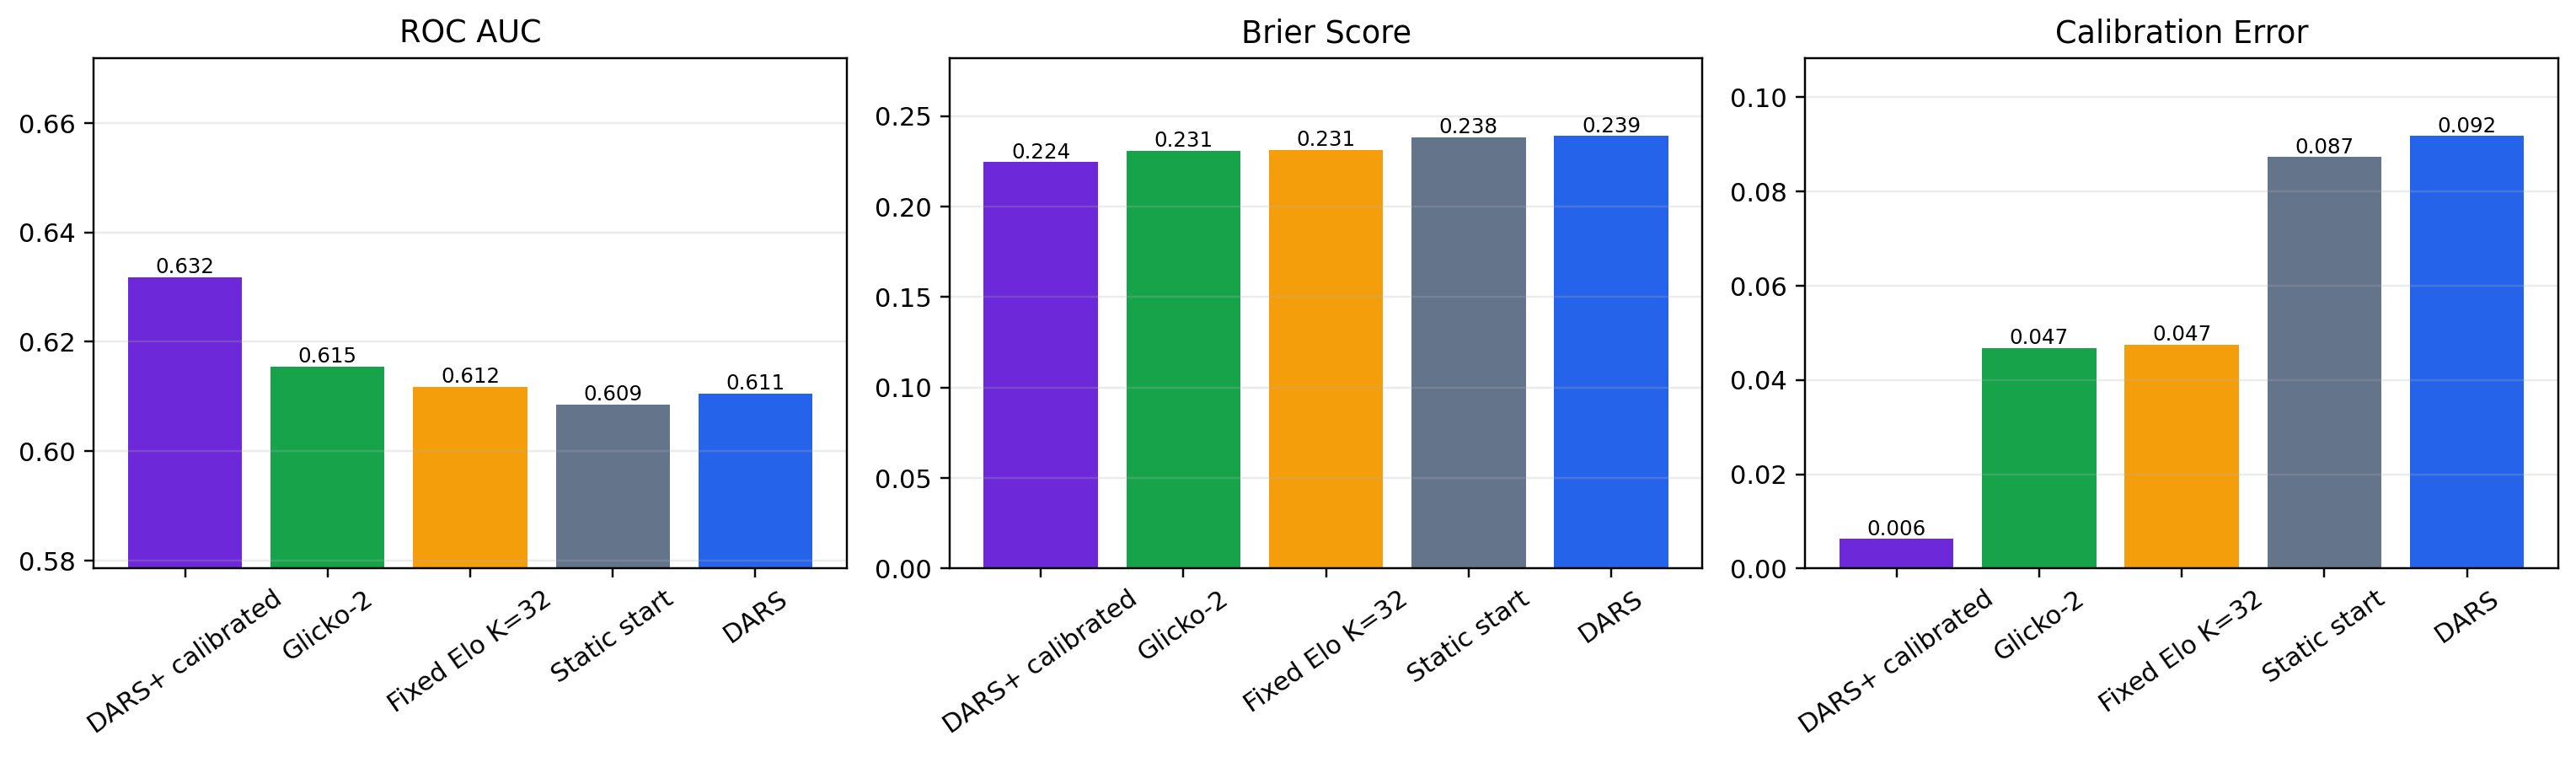
\includegraphics[width=\textwidth]{paper_figures/model_metric_comparison.png}
\caption{Held-out student benchmark visualization. DARS$^+$ gives the strongest AUC, lowest Brier score, and lowest calibration error.}
\label{fig:metrics}
\end{figure*}

DARS$^+$ improves Brier score over Glicko-2 by 0.0064 and over fixed Elo by 0.0068. The largest practical gain is calibration: DARS$^+$ ECE is 0.0062, compared with 0.0468 for Glicko-2 and 0.0475 for fixed Elo. This is important in an industry setting because teacher dashboards and readiness indicators depend on trustworthy probabilities, not only ranking quality.

\subsection{Bootstrap Intervals}
DARS$^+$ has ROC AUC mean 0.6320 with 95\% bootstrap interval [0.6255, 0.6385]. Glicko-2 has mean 0.6156 with interval [0.6070, 0.6221], and fixed Elo has mean 0.6125 with interval [0.6049, 0.6210].

\begin{figure}[t]
\centering
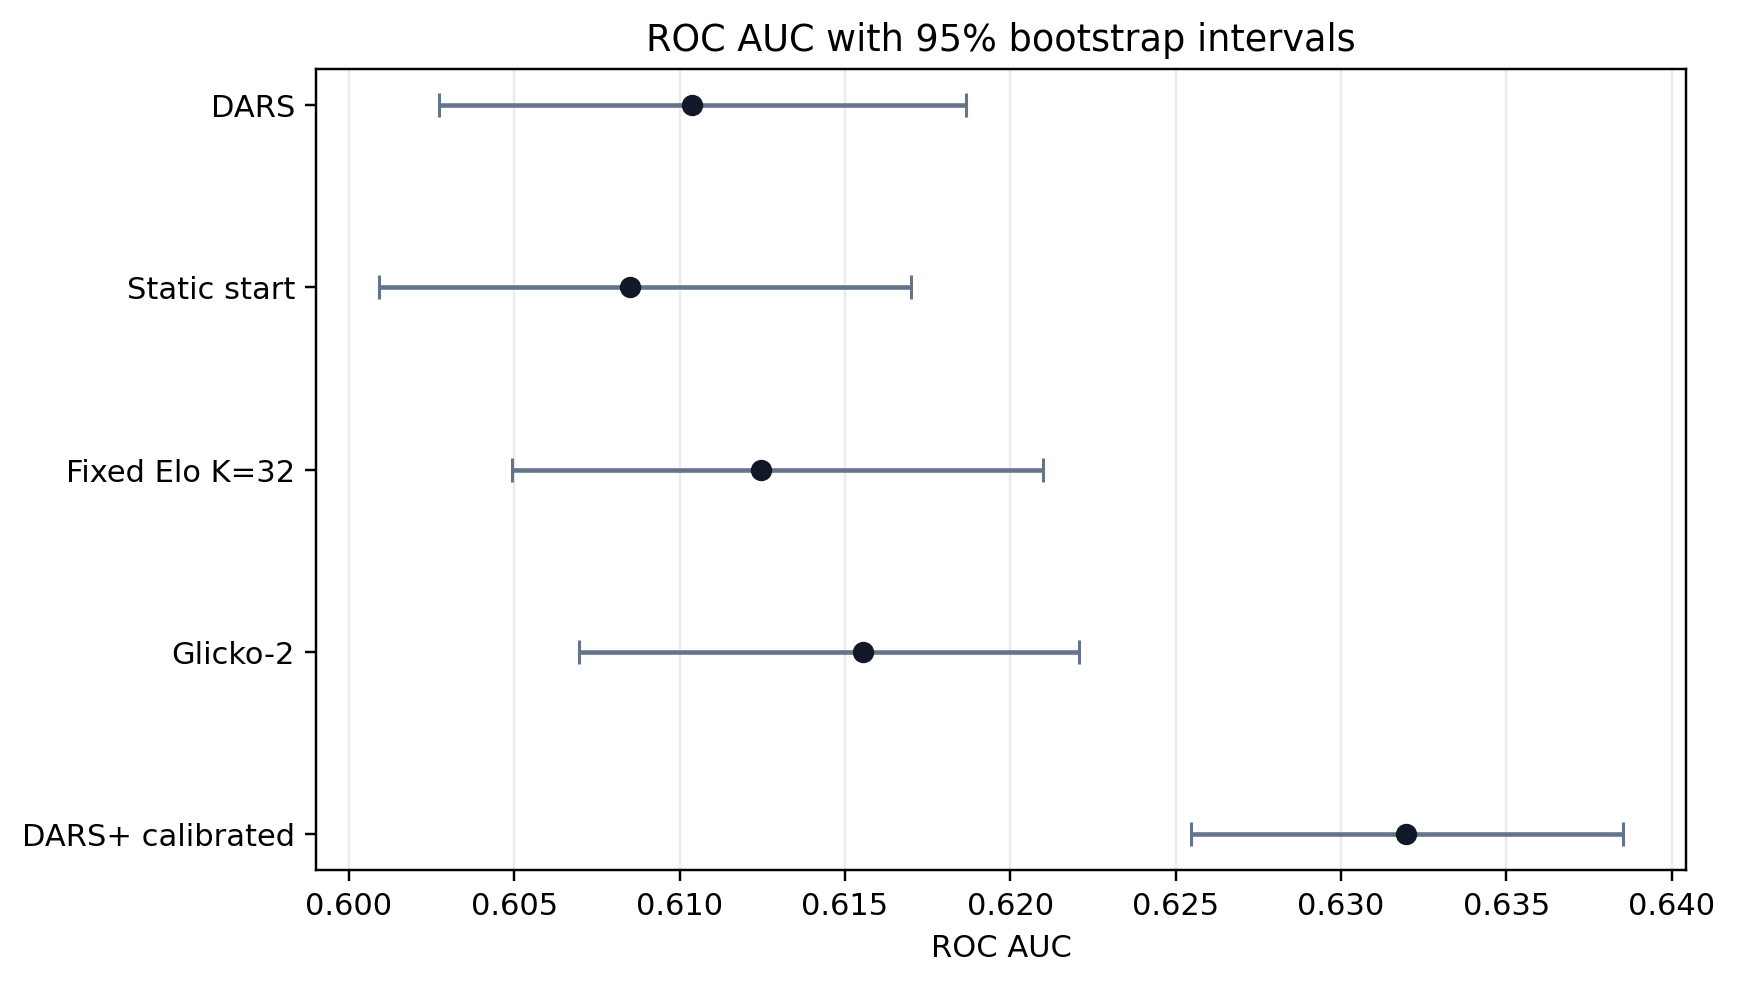
\includegraphics[width=\linewidth]{paper_figures/auc_bootstrap_intervals.png}
\caption{ROC AUC bootstrap intervals for implemented baselines.}
\label{fig:auc}
\end{figure}

\subsection{Temporal Validation}
Under the chronological per-student split, DARS$^+$ is trained on each student's earlier responses and evaluated on the final 30\%. On 21,104 test responses, DARS$^+$ achieves Brier 0.2166, log loss 0.6224, AUC 0.6422, and accuracy 0.6519. Raw DARS on the same temporal test set achieves Brier 0.2323, log loss 0.6705, AUC 0.6140, and accuracy 0.6405. This confirms that the calibrated feature layer improves future-response prediction without future leakage.

\subsection{Graph Routing and Remediation}
Graph-route recommendations dominate the served response volume and outperform fallback routes. Hop-1 graph-route questions reach 0.6201 accuracy over 67,708 attempts, while fallback routes range from 0.4526 to 0.5059 accuracy.

\begin{figure}[t]
\centering
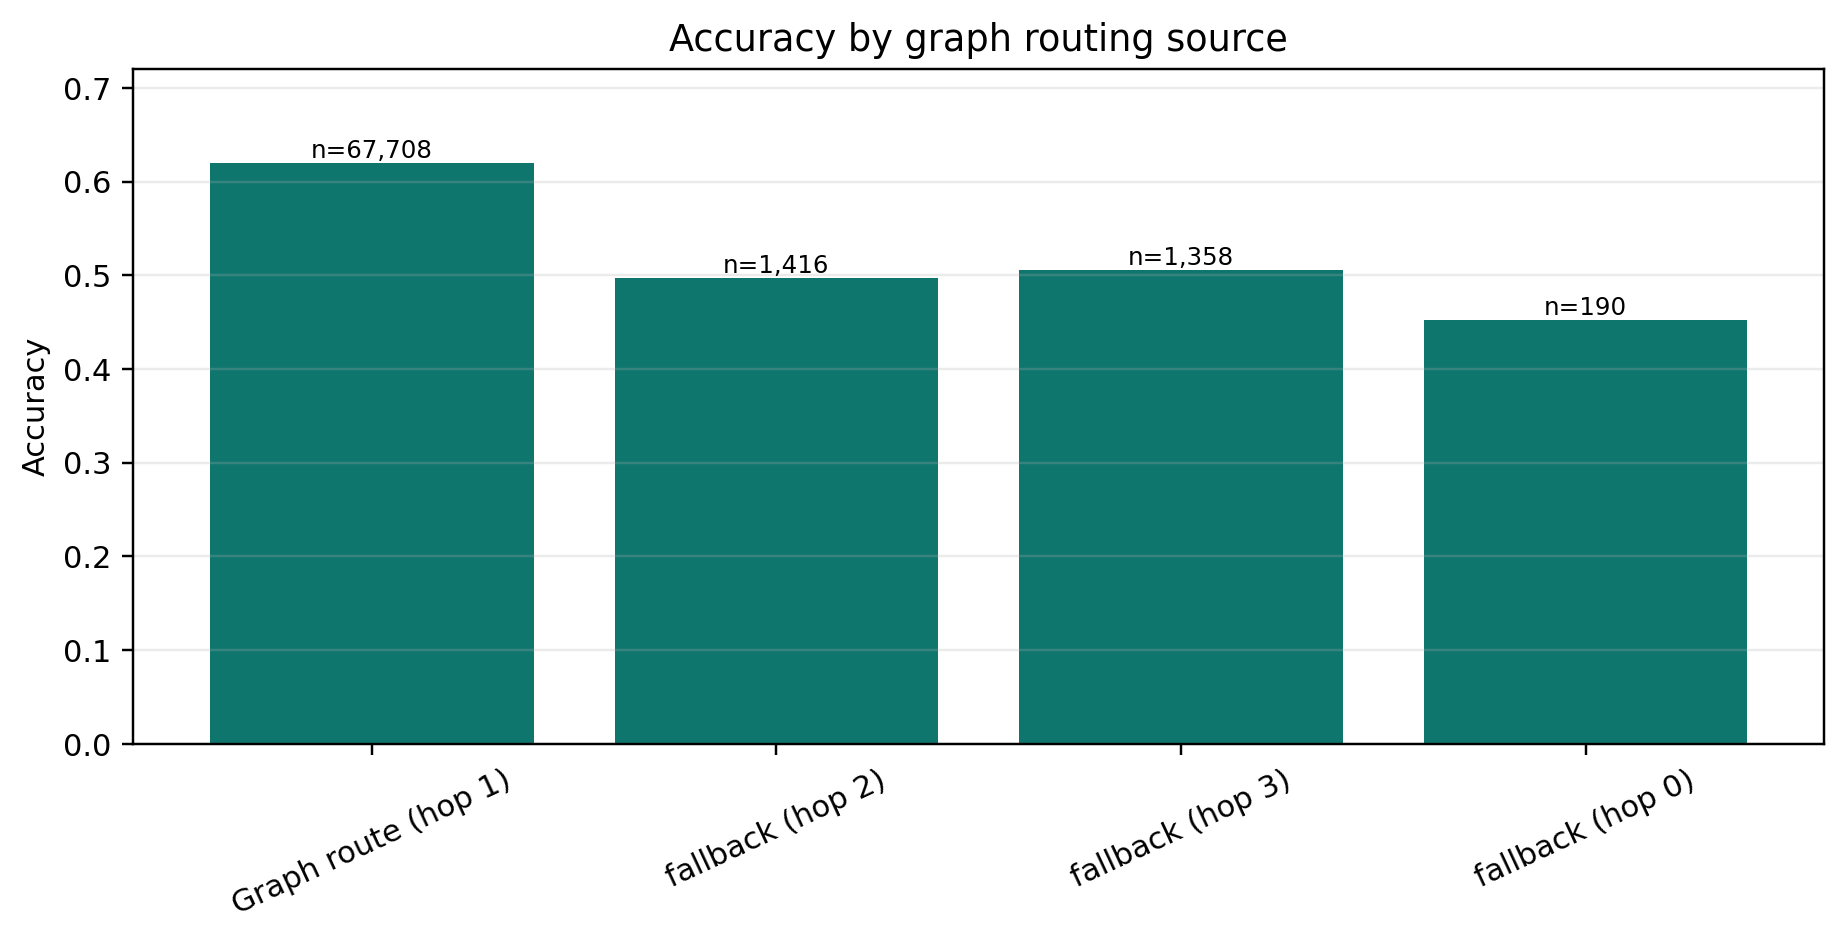
\includegraphics[width=\linewidth]{paper_figures/graph_route_accuracy.png}
\caption{Accuracy by recommendation source and graph hop distance.}
\label{fig:graph}
\end{figure}

Remediation attempts after missed questions reach 0.5912 accuracy over 25,980 attempts. Non-remediation next attempts after misses reach 0.5057 over 1,135 attempts. The same-topic recovery path rate is 0.9581, indicating that remediation remains conceptually local.

\begin{figure}[t]
\centering
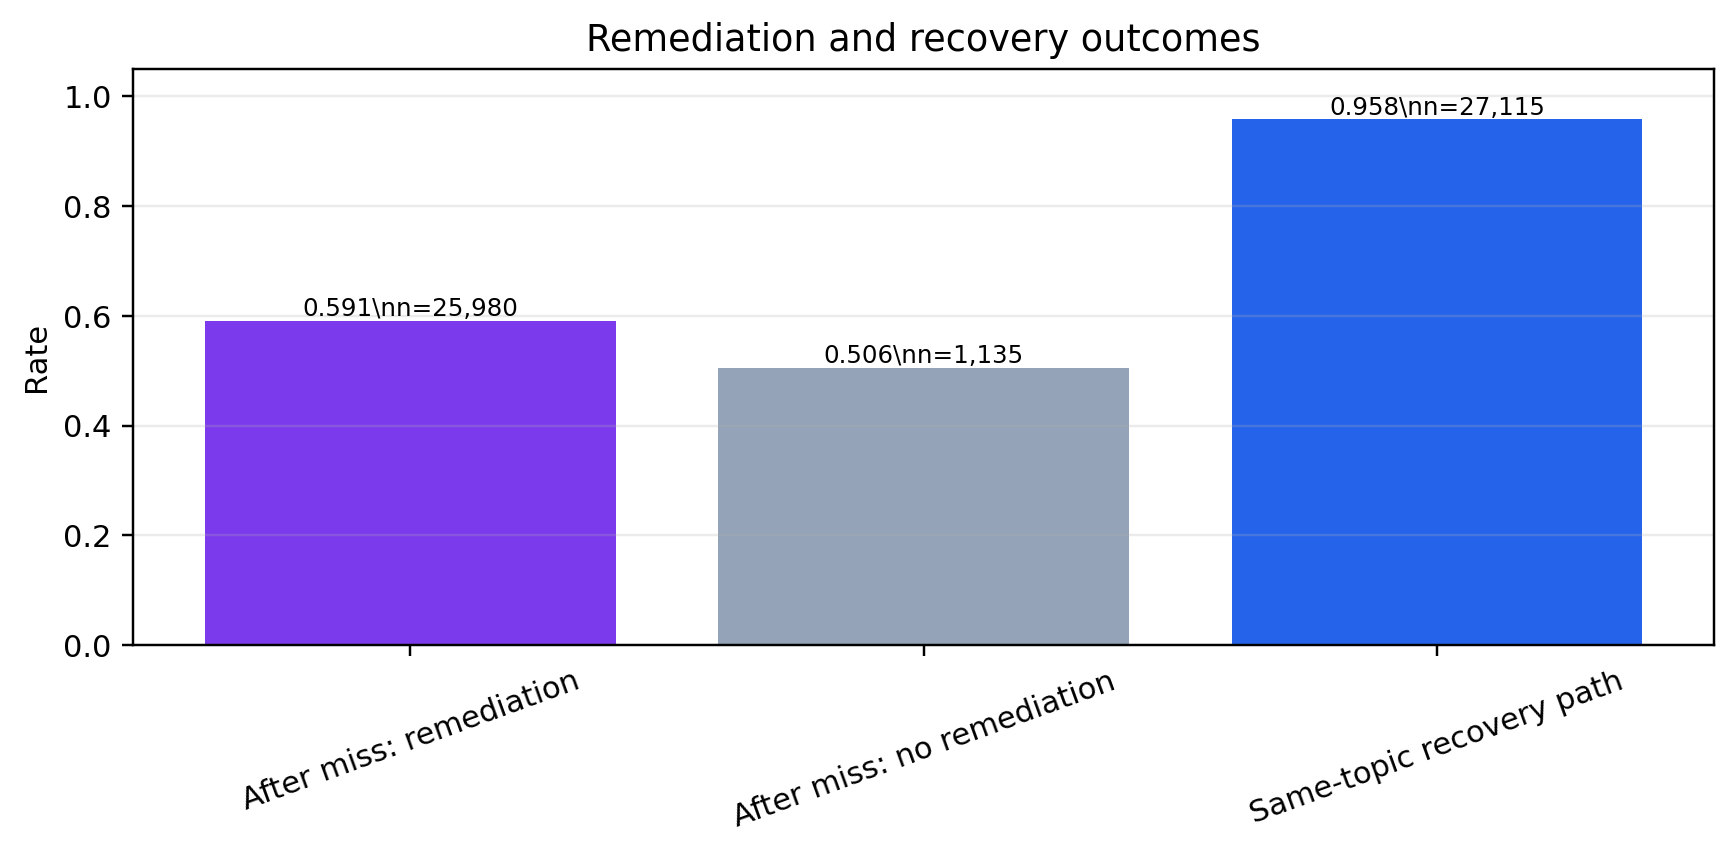
\includegraphics[width=\linewidth]{paper_figures/remediation_recovery.png}
\caption{Remediation and recovery outcomes after missed questions.}
\label{fig:remediation}
\end{figure}

\section{Industry Deployment Value}
The industry value of DARS is not limited to predictive accuracy. The implemented platform supports operational workflows that a deployed adaptive learning product needs:

\begin{itemize}[leftmargin=*]
  \item \textbf{Student workflows:} adaptive practice, test review, topic feedback, and recovery after misses.
  \item \textbf{Teacher workflows:} rosters, assignment grouping, student profiles, weak-topic analytics, and risk indicators.
  \item \textbf{Engineering workflows:} reproducible bot cohorts, CSV exports, notebook metrics, graph visualizations, and testable TypeScript modules.
  \item \textbf{Research workflows:} held-out student splits, temporal splits, baselines, calibration metrics, and bootstrap intervals.
\end{itemize}

This makes DARS suitable for an industry-track submission: it addresses a real product problem, implements a complete application stack, and produces measurable data-science impact.

\section{Literature Positioning}
\textbf{Dynamic Elo and adaptive $K$.} Vermeiren et al. show that fixed-$K$ Elo creates a stability-flexibility trade-off in adaptive learning, and that adaptive $K$ can respond to changing ability while reducing volatility~\cite{vermeiren2025dynamic}. DARS follows this line but extends the update with response quality, streaks, rapid-guess penalties, graph routing, and remediation flags.

\textbf{Deep Knowledge Tracing.} DKT introduced RNN-based student modeling and demonstrated that neural representations can improve prediction while avoiding explicit hand-coded knowledge structure~\cite{piech2015dkt}. DARS differs by prioritizing deployment interpretability and lightweight online updates. DKT remains an important future baseline for public datasets.

\textbf{Graph Knowledge Tracing.} GIKT argues that questions and skills form a relation graph, and that graph convolution can incorporate high-order question-skill correlations to reduce sparsity and improve prediction~\cite{yang2020gikt}. DARS is aligned with this motivation but uses the graph directly for recommendation, remediation, and feature calibration rather than end-to-end graph neural prediction.

\section{Limitations and Future Work}
The current evidence is based on simulated bot students. This is valuable for controlled engineering validation but must be extended to live learner logs before making strong educational effectiveness claims. The next stage should add:

\begin{itemize}[leftmargin=*]
  \item real classroom deployment data;
  \item public dataset benchmarks such as ASSISTments or Math Garden;
  \item DKT, SAKT, TrueSkill, and graph neural KT baselines;
  \item 5-fold cross-validation by student and 10 randomized trials;
  \item paired statistical tests and calibration reliability diagrams;
  \item expert validation of the question graph.
\end{itemize}

\section{Conclusion}
DARS provides an interpretable, deployment-ready adaptive rating and recommendation layer for GATEWay. It operationalizes recent ideas from dynamic Elo research, adds graph-aware remediation inspired by graph KT, and remains lightweight enough for a production web application. On the current 220-student bot benchmark, DARS$^+$ outperforms Glicko-2, fixed Elo, static rating, and raw DARS across prediction and calibration metrics. The project therefore contributes both an industry-ready adaptive assessment system and a reproducible research pipeline for future DSAA-level evaluation.

\begin{acks}
This submission draft was prepared from the GATEWay repository, generated DARS datasets, executed metrics notebooks, and the cited adaptive learning and knowledge tracing literature.
\end{acks}

\begin{thebibliography}{9}
\bibitem{vermeiren2025dynamic}
H. Vermeiren, A. D. Hofman, M. Bolsinova, H. L. J. van der Maas, and W. Van Den Noortgate.
\newblock Balancing stability and flexibility: investigating a dynamic K value approach for the Elo rating system in adaptive learning environments.
\newblock \emph{User Modeling and User-Adapted Interaction}, 36, Article 4, 2026. Published online 2025.
\newblock \url{https://doi.org/10.1007/s11257-025-09439-z}.

\bibitem{piech2015dkt}
C. Piech, J. Spencer, J. Huang, S. Ganguli, M. Sahami, L. Guibas, and J. Sohl-Dickstein.
\newblock Deep Knowledge Tracing.
\newblock arXiv:1506.05908, 2015.
\newblock \url{https://doi.org/10.48550/arXiv.1506.05908}.

\bibitem{yang2020gikt}
Y. Yang, J. Shen, Y. Qu, Y. Liu, K. Wang, Y. Zhu, W. Zhang, and Y. Yu.
\newblock GIKT: A Graph-based Interaction Model for Knowledge Tracing.
\newblock arXiv:2009.05991, 2020.
\newblock \url{https://arxiv.org/abs/2009.05991}.

\bibitem{elo}
A. E. Elo.
\newblock \emph{The Rating of Chessplayers, Past and Present}.
\newblock Arco, 1978.

\bibitem{glickman}
M. E. Glickman.
\newblock Example of the Glicko-2 System.
\newblock Technical note, 2022.

\bibitem{trueskill}
R. Herbrich, T. Minka, and T. Graepel.
\newblock TrueSkill: A Bayesian Skill Rating System.
\newblock In \emph{NeurIPS}, 2007.
\end{thebibliography}

\end{document}
